\newpage
\subsection{Fonctionnalité 3}
La fonctionnalité 3 permettra l'envoi de courriers électroniques aux établissements qui contiendront une lettre type accompagnée d'une plaquette en pièce jointe. La figure \ref{envoiMailsCibles} présentera le diagramme de cas d'utilisation concernant l'envoi d'emails ciblés aux établissements.\\
 La plaquette sera fonction du type d'établissement et envoyé au format pdf. Le corps de l'e-mail contiendra la lettre type. La figure \ref{fonctionnalite3MailType} présentera une maquette du courriel type envoyé aux établissements. Ce mail sera redéfini avec le client afin qu'il soit plus complet et plus attrayant.\\


\begin{figure}[H]
	\centering
	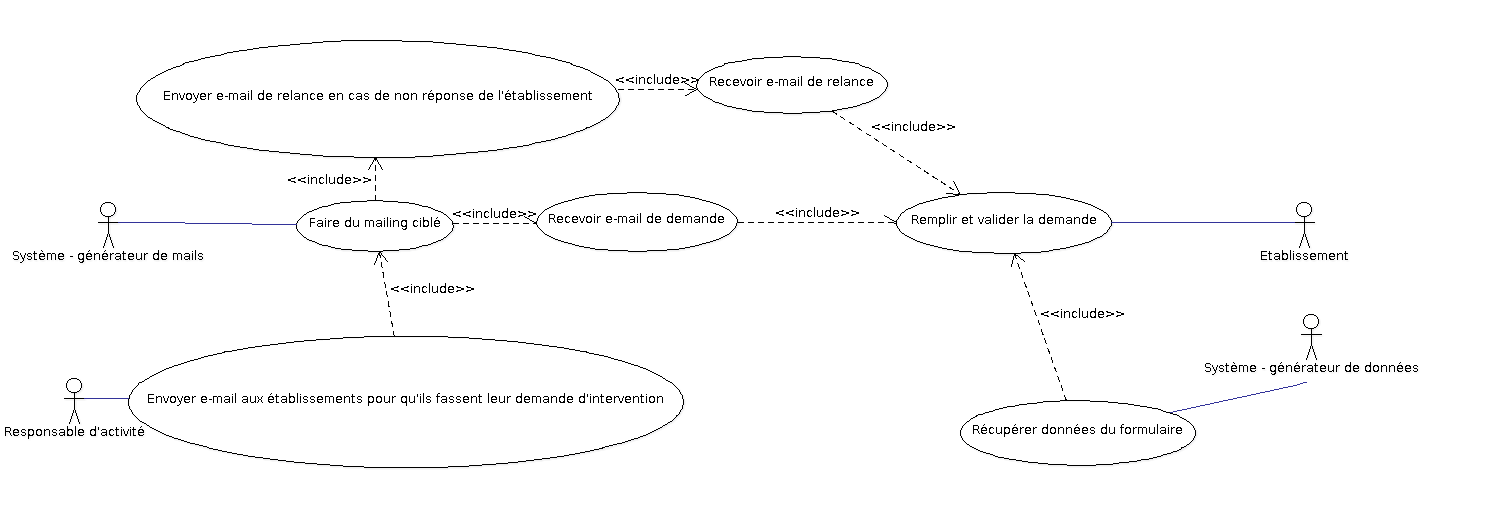
\includegraphics[scale=0.375]{images/casDUtilisation/fonctionnalite3Mailing.png}
	 \caption{Cas d'utilisation~: Envoyer des e-mails ciblés}
	 \label{envoiMailsCibles}
\end{figure}

% Figure : version 1.00, date 24/02/16, auteur Michel Cressant
\begin{figure}[H]
	\centering
	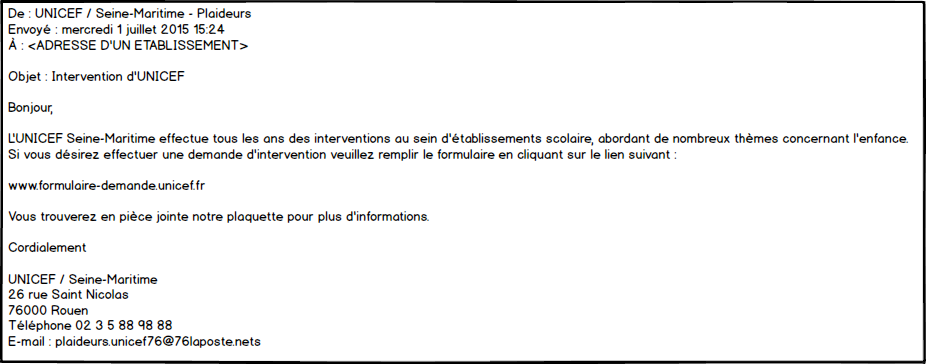
\includegraphics[scale=0.57]{images/maquettes/fonctionnalite3MailType}
	\caption{Maquette~: Email type envoyé aux établissement}
	\label{fonctionnalite3MailType}
\end{figure}


Cette fonctionnalité doit également permettre un envoi ciblé en fonction de plusieurs critères qui pourront être sélectionnés simultanément :
\begin{itemize}
\item le type de l'établissement (maternelle, élémentaire, centre de loisirs,...), 
\item la distance des villes suivantes : Rouen, Le Havre, Yvetot, Fécamp, Dieppe et Neuchâtel en Bray à la ville de l'établissement,
\item la non-réponse à une précédente sollicitation pour cette année scolaire (un mail de relance),
\item la réponse à une précédente sollicitation pour cette année scolaire (les établissements ayant demandé une action de frimousses ou une action ponctuelle mais pas de plaidoyer),
\item un sous-ensemble spécifique des adresses obtenues soit manuellement soit par l'application d'un critère (les écoles d'une ville donnée, un type donné par exemple),
\item exclure de la liste les établissements ayant fait une demande qui n'a pas pu être satisfaite par les plaideurs (pour des raisons d'emploi du temps, distance, ...). \\
\end{itemize}

Chaque e-mail invitera l'établissement à se connecter à un lien (actif) contenant un formulaire à remplir pour effectuer une demande d'intervention. Les champs à remplir seront : 
\begin{itemize}
\item la ville de l'établissement, 
\item le nom de l'établissement, 
\item le nom de la personne référente sur cette action, 
\item l'adresse électronique de la personne référente sur cette action ou celle de l'établissement si la personne  référente n'en a pas, 
\item le numéro de téléphone de la personne référente ou de l'établissement si la personne référente n'en a pas,
\item les plages de dates souhaitées pour l'intervention (date de début et date de fin),
\item les disponibilités (jours et les moments souhaités comme dans le formulaire actuel), 
\item le matériel disponible (vidéo projecteur, TBI, enceinte ou  aucun), 
\item le type de classes concernées (maternelle, élémentaire (ou centre de loisirs élémenaire), collège (ou centre de loisirs collège), lycée, enseignement supérieur)
\item le niveau de la classe, 
\item le thème dominant de l'intervention souhaité, 
\item le nombre d'élèves à préciser si plusieurs classes,
\item des remarques.
\end{itemize}
La figure \ref{fonctionnalite3FormulaireDeDemandeDInterventions} présentera une maquette du formulaire de demande d'intervention.
\newpage
% Figure : version 1.00, date 24/02/16, auteur Michel Cressant
\begin{figure}[H]
	\centering
	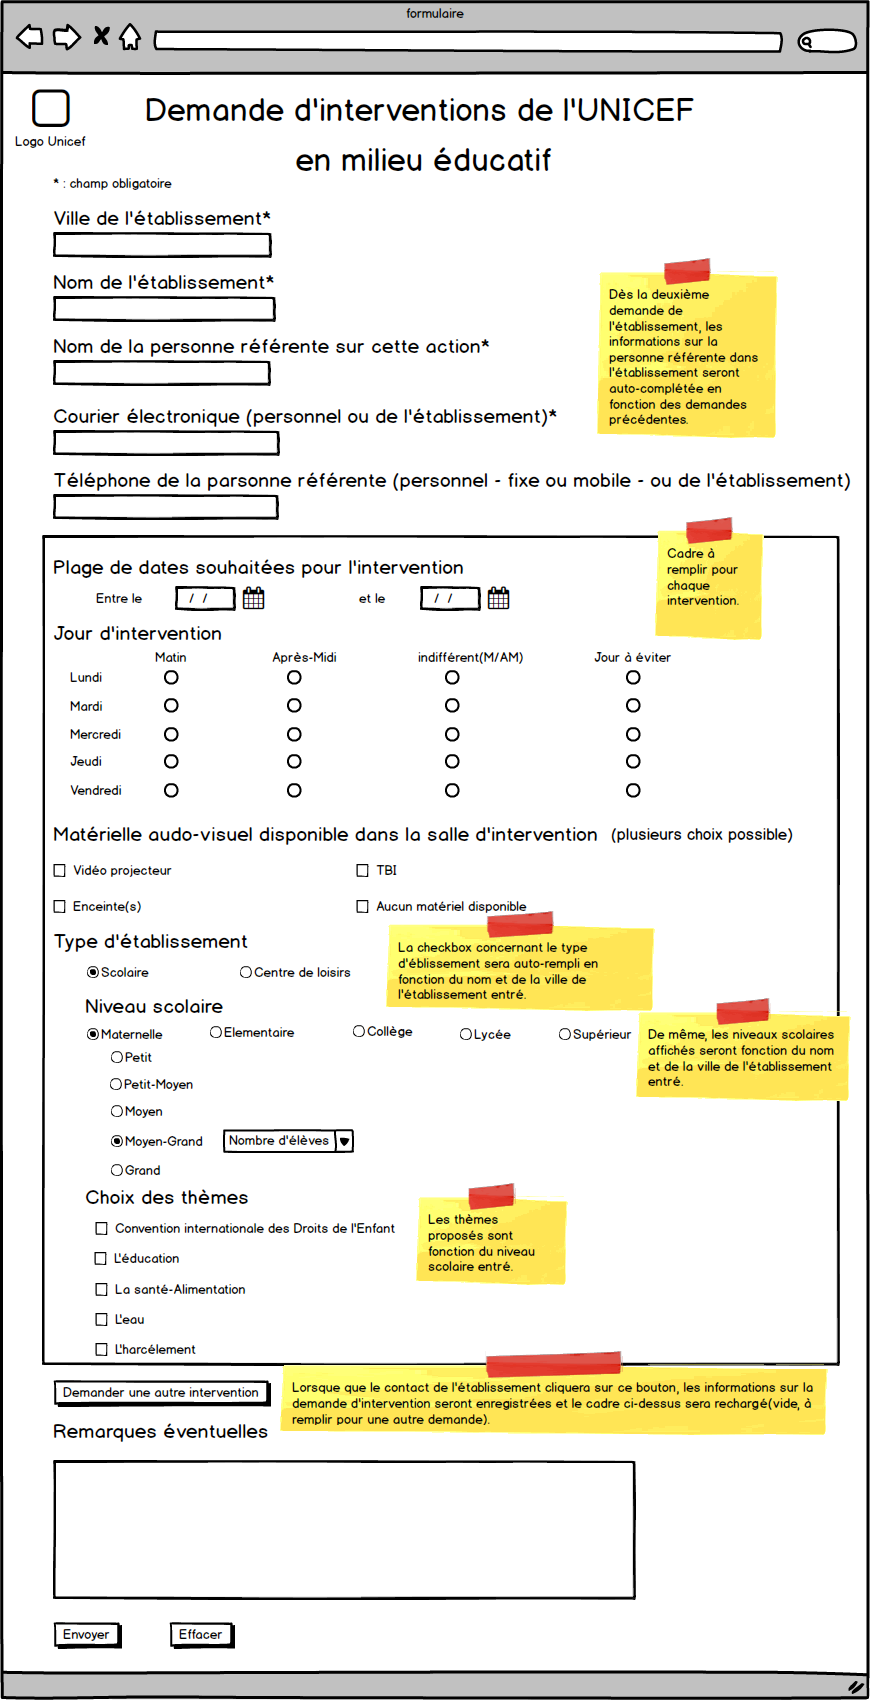
\includegraphics[scale=0.415]{images/maquettes/fonctionnalite3FormulaireDeDemandeDInterventions.png}
	\caption{Maquette~: Formulaire de demande d'intervention}
	\label{fonctionnalite3FormulaireDeDemandeDInterventions}
\end{figure}

Les réponses à ce formulaire viendront alimenter la base de données des demandes d'intervention. \\
Concernant le matériel disponible , plusieurs matériels pourront être choisis. \\
Concernant le niveau de la classe, nous reprendrons ceux proposés dans le formulaire actuel. Si la classe regroupe le niveau Grande Section et CP, l'information doit être précisée en remarque.
Concernant les classes spéciales (classe pour l'inclusion scolaire, sections d'enseignement général et professionnel adapté, etc...), elles ne seront pas traitées comme les classes par défaut, elles seront précisées dans le champs remarque.
\\
Les thèmes des interventions seront prédéfinis pour tous les établissements en fonction du comité dont les établissements dépendent.  